% !TeX root = main.tex
% !LW recipe = latexmk (presentation)
\documentclass[aspectratio=169,11pt,t]{beamer}
\usepackage{beamart}
\usepackage{quantikz}
\usepackage{booktabs}
\addbibresource{main.bib}

\title{Polynomial-time simulation of\\
  non-Clifford quantum error correction}
\presenter{Arthur Pesah}{FU Berlin}
\date{}                       % Set the talk date here.
\venue{}                      % Set the venue here.
\coauthors{%
  \coauthorportrait[yshift=-3mm]{assets/serban-cercelescu.png}
    {Serban Cercelescu}{Oxford}%
  \hspace{9mm}%
  \coauthorportrait[yshift=-4.5mm]{assets/mark-koch.jpg}{Mark Koch}{Oxford}%
}
\hypersetup{pdfauthor={Arthur Pesah},
  pdftitle={Polynomial-time simulation of non-Clifford quantum error correction}}

\setlength{\catchsentencewidth}{.7\paperwidth}

\arxivpaper[assets/qr-arxiv-transparent.png]{2610.06811}
\githubrepo[assets/qr-github-transparent.png]{mark-koch}{merlin-sim}

\begin{document}

\begin{frame}
  \titlepage
\end{frame}

% The sentence is defined once; <2>, <3>, ... select the highlighted term.
% This is example wording for the overview, ready to adapt as the talk develops.
\newcommand{\overviewSentence}{
  \catchterm<2>{Most magic-state preparation protocols} can be \catchterm<3>{simulated} in \catchterm<4>{polynomial-time}
}

% One Beamer frame produces four successive pages in the PDF.
\begin{frame}{Overview}
  \overviewstatement{\overviewSentence}

  \termexplanation{1}{Most magic-state preparation protocols}{%
      Circuits made of CNOT, $T$, Paulis, $Z$ measurements and \textit{compatible} $X$ measurements.
      \newline \newline
      \emphword{Examples}:
      \begin{itemize}
        \item Magic state distillation and cultivation based on applying a logical 3rd level non-Clifford gate to a code.
        \item Code switching between 3D and 2D codes.
      \end{itemize}
  }
  \termexplanation{2}{Simulated}{%
      Maintain state representation throughout the circuit.
      \newline
      Two representations: Schrödinger (phase polynomials) and Heisenberg (generalized stabilizer group).
      \newline \newline
      Can compute the following:
      \begin{itemize}
        \item Pauli expectation values and amplitudes
        \item Measurement samples
        \item State equality
      \end{itemize}

  }
  \termexplanation{3}{Polynomial time}{%
      Polynomial-time complexity in the number of qubits and circuit depth.

      No exponential dependence in the number of $T$ gates!

      No exponential in the number of logical qubits, in contrast to previous work\slidecite{surti2026efficient}.
  }
\end{frame}

\outlineslide

\sectionslide{The phase polynomial representation}

\begin{frame}{Phase-polynomial states}
    \emphword{Unitary gate set}: the third-order CNOT-dihedral group
    $G_3=\langle \text{CNOT}, T, X \rangle$\slidecite{cross2016scalable}

    \pause
    Commuting $T$ through the CNOTs: all diagonal non-Clifford gates of the third-level, i.e. $T$, $\text{CS}$, $\text{CCZ}$

    \pause
    \emphword{Initial state}: $\ket{0}^{\otimes \ell} \ket{+}^{\otimes m}$

    \pause
    \emphword{Question}: what happens when we apply $G_3$ gates to $\ket{0}^{\otimes \ell} \ket{+}^{\otimes m}$?
    $$
    U\ket{0}^{\otimes \ell} \ket{+}^{\otimes m} \propto \sum_{y\in \mathbb{F}_2^m} U \ket{x}
    $$
    with $\ket{x}= \ket{0}^{\otimes \ell} \ket{y}$

    \pause
    \emphword{New question}: what is $U \ket{x}$ for $U \in G_3$?
\end{frame}

\begin{frame}{Phase-polynomial states}
  \emphword{$X$ operators}:
  $X(b)\ket{x}=\ket{x+b}$

  \pause
  \emphword{CNOT operators}:
  $U_C\ket{x}=\ket{Ax}$

  \pause
  \emphword{Diagonal non-Clifford operators}: for $\omega=e^{i\pi/4}$, we have
  \newcommand{\diagonalGateActions}{%
    \begin{aligned}
      T_i\ket{x}&=\omega^{x_i}\ket{x} \\
      CS_{i,j}\ket{x}&=\omega^{2 x_i x_j}\ket{x} \\
      CCZ_{i,j,k}\ket{x}&=\omega^{4 x_i x_j x_k}\ket{x}
    \end{aligned}%
  }
  \[
    \diagonalGateActions
    \uncover<4->{%
      \left.\vphantom{\diagonalGateActions}\right\}
      \quad\Rightarrow\quad U_D\ket{x}=\omega^{f(x)}\ket{x}%
    }
  \]
  \uncover<4->{%
  for a so-called \emphword{third-order phase polynomial}:
  \[
    f(x)=\sum_{i} a_i x_i + 2 \sum_{i<j} b_{ij} x_i x_j + 4 \sum_{i<j<k} c_{ijk} x_i x_j x_k
  \]
  }
\end{frame}

\begin{frame}{Phase-polynomial states}
  \emphword{Therefore}, for $U\in G_3$ we have
  \[
    U \ket{x} = U_D X(b) U_C \ket{x} = \omega^{f(Ax+b)} \ket{Ax+b}
  \]

  \pause
  \emphword{Our state}: $U \in G_3$ applied to $\ket{0}^{\otimes \ell} \ket{+}^{\otimes m}$ gives
  \begin{align*}
    U\ket{0}^{\otimes \ell} \ket{+}^{\otimes m} &\propto \sum_{y\in \mathbb{F}_2^m} U \ket{0}^{\otimes \ell} \ket{y} \\
    & \uncover<3->{\propto \sum_{y\in \mathbb{F}_2^m} \omega^{f(A\tilde{y}+b)} \ket{A\tilde{y}+b} \quad \text{ with } \tilde{y} = (0, y)} \\
    & \uncover<4->{\propto \sum_{x \in S} \omega^{q(x)} \ket{x}}
  \end{align*}
  \uncover<4->{with $S$ an affine subspace of $\mathbb{F}_2^{n+m}$ and $q$ a third-order phase polynomial.}
\end{frame}

\begin{frame}{Phase-polynomial states}
  \emphword{Definition (3PP state)}: a third-order phase polynomial (3PP) state is a state of the form
  \[
    \ket{\psi} \propto \sum_{x\in S} \omega^{q(x)} \ket{x}
  \]
  with $S$ an affine subspace and $q$ a third-order phase polynomial.

  \pause
  \emphword{Property}: 3PP states are efficient to store
  \begin{itemize}
    \item $O(N^2)$ parameters for $S$ (generator matrix and offset)
    \item $O(N^3)$ parameters for $q$ (coefficients of the polynomial)
  \end{itemize}

  \pause
  \emphword{Claim}: also efficient to update under CNOT-dihedral gates

  \pause
  \emphword{Question}: but what about measurements?
\end{frame}

\sectionslide{Compatible measurements}

\begin{frame}{Compatible measurements: $Z$ measurements}
  \emphword{Definition (compatible measurement)}: the measurement of 3PP state $\ket{\psi}$ is \emphword{compatible} with $\ket{\psi}$
  if the post-measurement state is still a 3PP state (for every measurement outcome).

  \pause
  \emphword{Theorem}: $Z$ measurements are always compatible.

  \pause
  \emphword{Proof}: we apply the projector $\Pi^\mu=\frac{1}{2}(I+(-1)^\mu Z(v))$ to a 3PP state $\ket{\psi}$:
  \begin{align*}
    \Pi_\mu \ket{\psi}
    \propto
      \sum_{x\in S} \omega^{q(x)}\ket{x} + \sum_{x\in S} \omega^{q(x)}(-1)^\mu Z(v) \ket{x}
  \end{align*}
  \pause
  Using $Z(v)\ket{x}=(-1)^{v\cdot x}\ket{x}$, we get:
  \begin{align*}
    \Pi_\mu \ket{\psi} \propto
      \sum_{x\in S} \omega^{q(x)} (1 + (-1)^{\mu + v\cdot x}) \ket{x}
  \end{align*}
  \pause
  $\Rightarrow$ Doesn't change the phase polynomial, but reduces the support to $S\cap\{x:v\cdot x=\mu\}$.

  \pause
  $\Rightarrow$ Still a 3PP state!
\end{frame}

\begin{frame}{Compatible measurements: $X$ measurements}
  \emphword{Observation 1}: not every $X$ measurement can be compatible.

  Otherwise, we would get universality through a measurement-based Hadamard gadget:

  {\centering
  \begin{quantikz}[column sep=3mm,row sep=3mm]
    \lstick{$\ket{\psi}$} & \ctrl{1} & \meter{X} & \cwbend{1} \\
    \lstick{$\ket{+}$} & \control{} & \qw & \gate{X} & \rstick{$H\ket{\psi}$}\qw
  \end{quantikz}\par}\vspace{-2mm}

  \pause
  \emphword{Observation 2}: compatibility depends on the state.

  \pause
  For the Hadamard gadget, with $\ket{T}=T\ket{+}$:
  \[
    H\ket{0}=\ket{+}\quad\text{(compatible)},\qquad
    H\ket{T}\propto
    \cos\tfrac{\pi}{8}\ket{0}-i\sin\tfrac{\pi}{8}\ket{1}
    \quad\text{(incompatible)}.
  \]
  The latter has unequal amplitude magnitudes, so it is not a 3PP state.

  \pause
  \emphword{Question}: which $X$ measurements are compatible with a state
  $\ket{\psi}$ specified by $(S,q(x))$?
\end{frame}

\begin{frame}{Compatible $X$ measurements: support and phase}
  \emphword{Claim}: compatibility of measuring $X(v)$ is determined by whether
  $S=S+v$ and, if so, by the form of
  $\Delta_v q(x)=q(x+v)-q(x)\pmod 8$ on $S$.

  \pause
  \emphword{Indeed:} applying $\Pi_\mu=\frac12(I+(-1)^\mu X(v))$ gives
  \[
    \Pi_\mu\ket{\psi}\propto
      \sum_{x\in S}\omega^{q(x)}\ket{x}
      +(-1)^\mu\sum_{x\in S}\omega^{q(x)}\ket{x+v}.
  \]

  \pause
  \emphword{If $S\ne S+v$}: the two copies are disjoint, so there is no interference.
  Their union is affine and the relative sign adds an affine phase.
  $\Rightarrow$ Always compatible!

  \pause
  \emphword{If $S=S+v$}: relabeling the second sum gives
  \begin{align*}
    \Pi_\mu\ket{\psi}
    &\propto
    \sum_{x\in S}\bigl(\omega^{q(x)} + (-1)^\mu \omega^{q(x+v)}\bigr) \ket{x} \\
    &\propto
    \sum_{x\in S}\omega^{q(x)}\bigl(1+ \omega^{\Delta_v q(x) + 4\mu}\bigr)\ket{x}
  \end{align*}
\end{frame}


\begin{frame}{Classification of compatible $X$ measurements}
  \setlength{\parskip}{4bp}
  \emphword{Theorem}: measuring $X(v)$ on a 3PP state $(S,q)$ is compatible iff
  \begin{enumerate}
    \item $S\ne S+v$, or
    \item $S=S+v$ and one of the following holds on $S$ (modulo $8$):
  \end{enumerate}
  \[
    \begin{aligned}
      \text{\emphword{(2a)}}\quad \Delta_v q(x)&=4f(x),
        &&f\text{ affine},\\
      \text{\emphword{(2b)}}\quad \Delta_v q(x)&=2+4g(x),
        &&2g\text{ a third-order phase polynomial},\\
      \text{\emphword{(2c)}}\quad \Delta_v q(x)&=(-1)^{h(x)}d,
        &&h\text{ affine},\quad d\in\{1,3,5,7\}.
    \end{aligned}
  \]

  \pause
  \emphword{Example 1 (deterministic measurement)}:
  $X(v)\ket{\psi}=(-1)^\mu\ket{\psi}$ $\;\Rightarrow\;$ case (2a).

  \pause
  \emphword{Proof}: $X(v)$ shifts the support, so $S+v=S$.
  Matching amplitudes at $x\in S$ gives
  \[
    \omega^{q(x+v)}=(-1)^\mu\omega^{q(x)}
    \;\Rightarrow\; q(x+v)= q(x)+4\mu\pmod 8 \;\Rightarrow\; \Delta_v q(x)=4\mu\pmod 8.
  \]
  Thus $\Delta_v q=4f$ with $f(x)=\mu$ constant, hence affine: case (2a).
\end{frame}

\begin{frame}{Classification of compatible $X$ measurements}
  \setlength{\parskip}{4bp}
  \emphword{Theorem}: measuring $X(v)$ on a 3PP state $(S,q)$ is compatible iff
  \begin{enumerate}
    \item $S\ne S+v$, or
    \item $S=S+v$ and one of the following holds on $S$ (modulo $8$):
  \end{enumerate}
  \[
    \begin{aligned}
      \text{\emphword{(2a)}}\quad \Delta_v q(x)&=4f(x),
        &&f\text{ affine},\\
      \text{\emphword{(2b)}}\quad \Delta_v q(x)&=2+4g(x),
        &&2g\text{ a third-order phase polynomial},\\
      \text{\emphword{(2c)}}\quad \Delta_v q(x)&=(-1)^{h(x)}d,
        &&h\text{ affine},\quad d\in\{1,3,5,7\}.
    \end{aligned}
  \]

  \emphword{Example 2 (anticommuting $Z$ stabilizer)}:
  if $Z(w)\ket{\psi}=\ket{\psi}$ and $Z(w)$ anticommutes with $X(v)$,
  measuring $X(v)$ is compatible: case (1).

  \pause
  \emphword{Proof}: for $x \in S$, $Z(w)\ket{\psi}=\ket{\psi}$ gives $w\cdot x=0$. Anticommutation gives
  $w\cdot v=1$. Thus:
  \[
    w\cdot(x+v)=0+1\ne 0 \pmod 2
    \;\Rightarrow\; x+v \notin S \;\Rightarrow\; S \neq S+v.
  \]
\end{frame}

\begin{frame}{Application to quantum error correction}
  \emphword{Problem}: we need to look at the compatibility of QEC measurements with \emphword{noisy} states.

  \pause
  \emphword{Question}: what noise model should we consider?

  \pause
  \emphword{Observation 1}: in a CNOT-dihedral circuit (i.e. $X$,$T$,CNOT), Pauli errors propagate into \emphword{diagonal Clifford and Pauli (DCP)} gates. Example:
  \begin{itemize}
    \item $TXT^\dagger = e^{-i\pi/4} S X$
    \item $(\text{CCZ}) X (\text{CCZ})^\dag = X \; \text{CZ}$
  \end{itemize}

  \pause
  \emphword{Observation 2}: CNOT-dihedral circuits preserve DCP errors. Indeed:
  \begin{enumerate}
    \item Pauli part of the DCP error: propagate into a new DCP operator
    \item Diagonal part of the DCP error: turn into another diagonal operator (due to CNOTs)
  \end{enumerate}

  \pause
  \emphword{Noise model}: DCP errors at every circuit location
\end{frame}



\begin{frame}{Application to quantum error correction}
  \emphword{Theorem (measurement compatibility under noise)}: assume
  \begin{enumerate}
    \item Circuit made of CNOT-dihedral gates and compatible measurements
    \item Every ideal $X$ measurement is either deterministic, or anticommutes with a current $Z$ stabilizer
  \end{enumerate}
  Then, all measurements remain compatible under arbitrary inserted DCP faults.

  \pause
  \emphword{Examples}:
  \begin{itemize}
    \item \emphword{Distillation and non-Clifford computation}: logical
      CNOT-dihedral gates on CSS codes, followed by ideally deterministic checks.
    \item \emphword{DCP checks in cultivation}: controlled-DCP gates give deterministic ancilla $X$ readouts.
    \item \emphword{CSS gauge fixing and code switching}: new $X$ checks are
      fixed or anticommute with a current $Z$ constraint.
  \end{itemize}
\end{frame}

\sectionslide{DCP stabilizer formalism}

\begin{frame}{DCP stabilizer formalism}
  \emphword{Question}: can we come up with a stabilizer picture for

  \pause
  \emphword{Observation}: if we start with a state stabilized by a Pauli operator $S$, and apply a gate $U \in G_3$, then the new state is stabilized by $S'=U S U^\dag$, \emphword{which is a DCP operator}.
  \newline
  $\Rightarrow$ Let's look at states uniquely stabilized by a group of DCP operators. We call these \emphword{DCP states}.

  \pause
  \emphword{Example}: $\ket{00}$ is stabilized by
  $\mathcal{S}_{\text{DCP}} = \langle S_1, S_2, \text{CZ}_{12} \rangle$. Interestingly:
  \begin{enumerate}
    \item It has $m=3$ independent generators, but $n=2$ qubits. Contrasts with Pauli case, where $n=m$.
    \item However, also uniquely stabilized by some dim-$2$ subgroups of $\mathcal{S}_{\text{DCP}}$: $\langle Z_1, Z_2 \rangle$, $\langle Z_1, S_2 \rangle$, etc.
  \end{enumerate}

  \emphword{Questions}:
  \begin{enumerate}
    \item What is the link between DCP states and 3PP states?
    \item Is every DCP state uniquely stabilized by an $n$-dimensional DCP subgroup?
    \item Can we build a \textit{DCP tableau simulator}, with update rules for compatible measurements?
  \end{enumerate}
\end{frame}

\begin{frame}{DCP stabilizer formalism}
  \emphword{Question 1}: what is the link between DCP states and 3PP states? \pause \emphword{They're the same!}

  \pause
  \emphword{3PP states are DCP states}:
  \begin{enumerate}
    \item Every 3PP state can be written as $\ket{\psi}=U\bigl(\ket{0}^{\otimes \ell}\ket{+}^{\otimes m}\bigr)$ for some $U\in G_3$.
    \item $\ket{0}^{\otimes \ell}\ket{+}^{\otimes m}$ is uniquely stabilized by $\langle Z_1,\ldots,Z_\ell,X_{\ell+1},\ldots,X_{\ell+m} \rangle$.
    \item $\ket{\psi}$ is stabilized by the DCP operators $\langle U Z_1 U^\dag,\ldots,U Z_\ell U^\dag,U X_{\ell+1} U^\dag,\ldots,U X_{\ell+m} U^\dag \rangle$, and one can prove it's unique.
  \end{enumerate}


  \pause
  \emphword{DCP states are 3PP states}: let $G$ the DCP stabilizer group of $\ket{\psi}$. We note its $X$-part as:
  \[
    X(G)=\{v:DX(v)\in G\text{ for some diagonal }D\}.
  \]

  \emphword{Support}: $S=x_0+X(G)$, for a vector $x_0$ fixed by the diagonal stabilizers.

  \pause
  \emphword{Phases}: the diagonal factor in $DX(v)$ fixes the relative phase
  between $x$ and $x+v$.
\end{frame}

\begin{frame}{DCP stabilizer formalism}
  \emphword{Question 2}: is every DCP state uniquely stabilized by an $n$-dimensional DCP subgroup? \pause \emphword{Yes!}

  \pause
  By the equivalence with 3PP states,
  every DCP state is uniquely stabilized by
  \[
    \langle U Z_1 U^\dag,\ldots,U Z_\ell U^\dag,U X_{\ell+1} U^\dag,\ldots,U X_{\ell+m} U^\dag \rangle
  \]

  \pause
  \emphword{Question 3}: can we build a \textit{DCP tableau simulator}, with update rules for compatible measurements?

  \pause
  \emphword{Unitary gates}: conjugate each generator.

  \pause
  \emphword{$Z$ measurements}: DCP operators commute or anticommute with $Z(w)$.
  Keep commuting stabilizers and add the measured $\pm Z(w)$, as for Paulis.
  Deterministic outcomes leave the state unchanged.

  \pause
  \emphword{$X$ measurements}: apply 3PP state compatibility conditions with $S=x_0+X(G)$ and $\Delta_v q(x)=-d(x)\pmod 8$, where $d(x)$ is the diagonal factor in $DX(v)\in G$, i.e. $D\ket{x}=\omega^{d(x)}\ket{x}$.

  \pause
  \emphword{Therefore}: compatibility tests and tableau updates take polynomial time.
\end{frame}

\sectionslide{Benchmarking our simulator}

\begin{frame}{MERLIN: from theory to benchmarks}
  \setlength{\parskip}{2bp}
  \emphword{MERLIN}: our open-source simulator for non-Clifford QEC

  \emphword{Input}: Stim-like circuit descriptions.

  \pause
  \emphword{Benchmark circuits}:
  \begin{itemize}
    \item Bravyi--Haah distillation: $3k+8\to k$ magic states, increasing $k$.
    \item 15-to-1 distillation and distance-3 / distance-5 cultivation.
    \item $\mathrm{CCZ}$ code switching with $[\![27,3,3]\!]$ and $[\![81,3,5]\!]$ codes\slidecite{li2026transversal}.
  \end{itemize}

  \pause
  \emphword{Comparison}: Tsim\slidecite{haenel2026tsim},
  Xtim\slidecite{surti2026efficient}, Clifft\slidecite{chase2026clifft}
  and SymFT\slidecite{fang2026symft}.

  \pause
  \emphword{Metrics}: total runtime, sampling time per shot and peak memory.
\end{frame}

\begin{frame}{Bravyi--Haah: scaling with logical outputs}
  \centering
  
\includegraphics[width=.78\linewidth]{assets/bh-total-time.pdf-legend.pdf}\par
  \vspace{-2mm}
  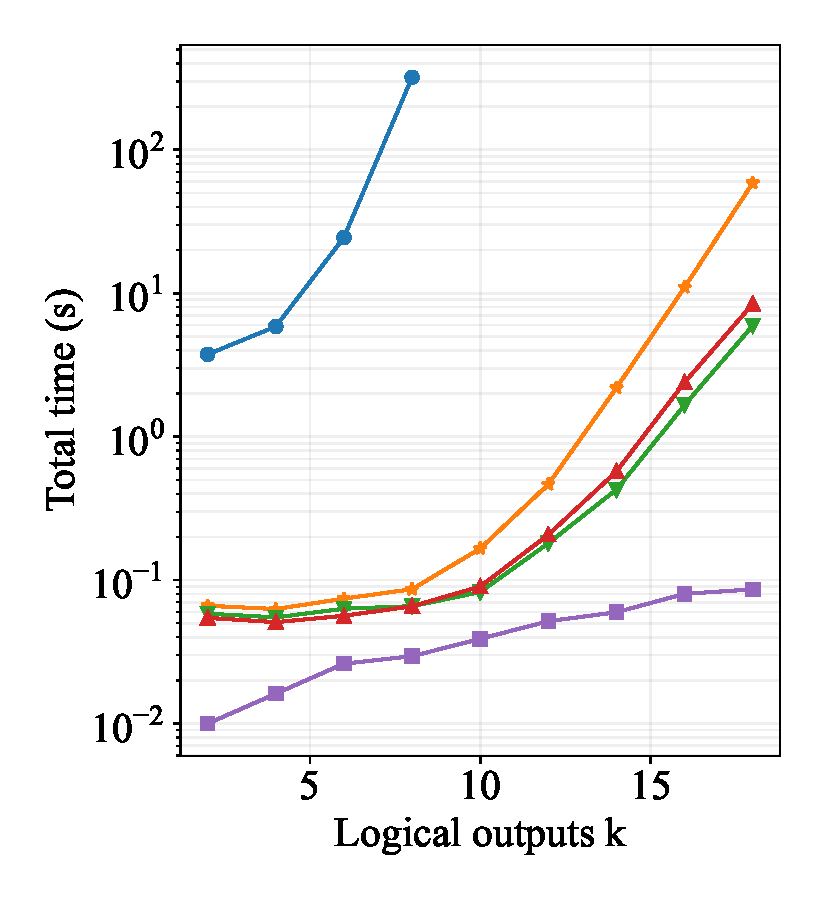
\includegraphics[width=.325\linewidth]{assets/bh-total-time.pdf}\hfill%
  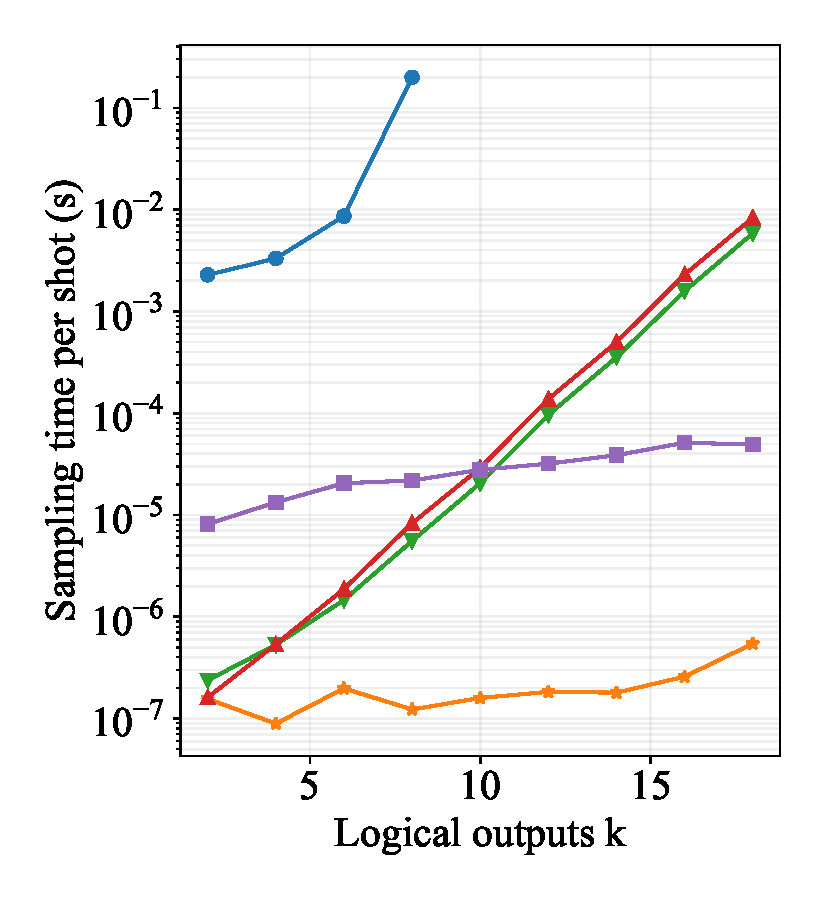
\includegraphics[width=.325\linewidth]{assets/bh-sample-time.pdf}\hfill%
  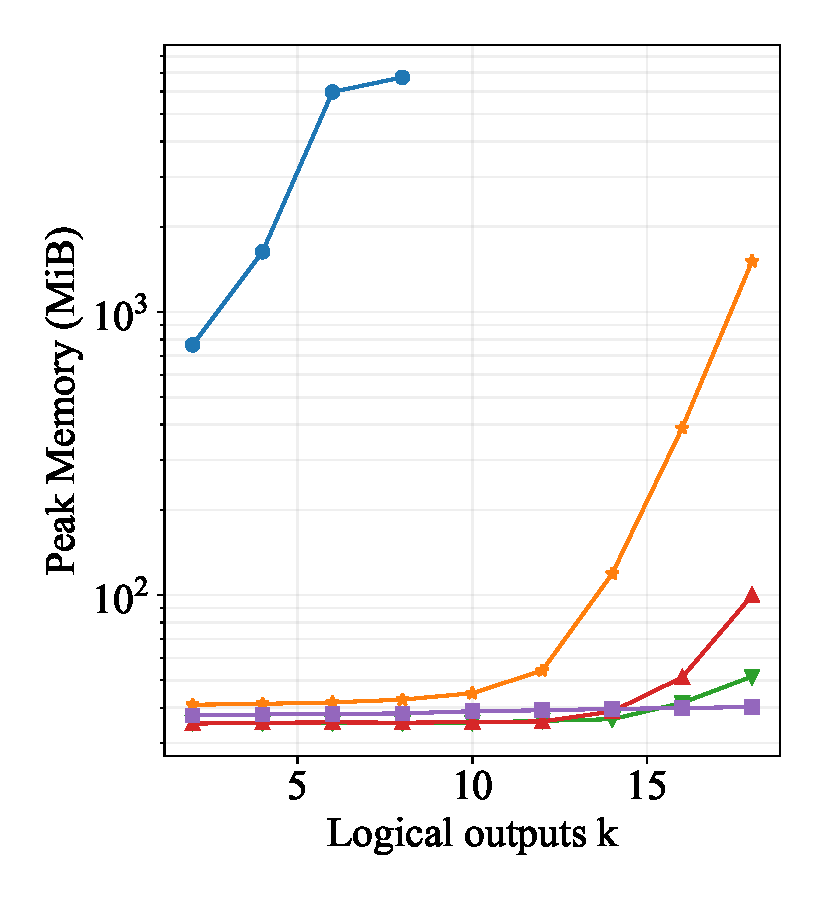
\includegraphics[width=.325\linewidth]{assets/bh-memory.pdf}\par
  \vspace{-1mm}
  {\fontsize{8}{10}\selectfont
    $1000$ attempted shots, $p=10^{-3}$.\par
    Total includes pre-processing. Sampling time excludes pre-processing.\par}
\end{frame}

\begin{frame}{Distillation, cultivation and code switching}
  \centering
  % \setlength{\parskip}{0pt}
  \setlength{\tabcolsep}{9pt}
  \renewcommand{\arraystretch}{.95}
  {\fontsize{8.5}{10}\selectfont
  \emphword{Total runtime in ms, including pre-processing}
  \begin{tabular}{lrrrrr}
    \toprule
    Circuit & Tsim & Xtim & Clifft & SymFT & \emphword{MERLIN} \\
    \midrule
    15-to-1  & 5029.95 & 85.86 & 99.56 & 57.67 & \textbf{12.52} \\
    Cultiv-3 & OOM & 65.29 & 54.29 & 63.63 & \textbf{28.98} \\
    Cultiv-5 & OOM & 253.51 & \textbf{67.93} & 577.20 & 202.01 \\
    Switch-3 & OOM & 2817.53 & OOM & ERR & \textbf{573.69} \\
    Switch-5 & OOM & OOM & OOM & ERR & \textbf{6959.13} \\
    \bottomrule
  \end{tabular}\par
  \vspace{1.5mm}
  \emphword{Time per shot in $\mu$s, excluding pre-processing}
  \begin{tabular}{lrrrrr}
    \toprule
    Circuit & Tsim & Xtim & Clifft & SymFT & \emphword{MERLIN} \\
    \midrule
    15-to-1  & 3446.85 & 0.40 & 0.37 & \textbf{0.18} & 9.62 \\
    Cultiv-3 & OOM & 0.39 & 0.51 & \textbf{0.34} & 28.34 \\
    Cultiv-5 & OOM & 7.70 & 7.97 & \textbf{6.52} & 200.15 \\
    Switch-3 & OOM & \textbf{2.65} & OOM & ERR & 549.93 \\
    Switch-5 & OOM & OOM & OOM & ERR & \textbf{6704.94} \\
    \bottomrule
  \end{tabular}\par}
  \vspace{1mm}
  {\fontsize{7}{9}\selectfont
  $1000$ attempted shots, $p=10^{-3}$. Cultivation excludes the escape stage.\newline
  OOM = allocation above 20 GB. ERR = runtime error. Cultiv / Switch suffix = distance.\par}
\end{frame}

\begin{frame}{Discussion: summary}
  \emphword{In summary}:
  \begin{enumerate}
    \item We have shown that CNOT-dihedral gates generate a class of states, which can be characterized by polynomial phases in the Schödinger picture, and DCP stabilizers in the Heisenberg picture.
    \pause
    \item We have classified all the measurements that are compatible with this class, making it useful for QEC.
    \pause
    \item We have implemented a simulator, MERLIN, that can simulate these circuits in polynomial time, and benchmarked it against other simulators.
  \end{enumerate}
\end{frame}

\begin{frame}{Discussion: parallel work}
  \setbeamerfont{itemize/enumerate body}{size=\fontsize{9bp}{12bp}}
  Lots of parallel work on the same topic, with different emphases and approaches:
  \begin{enumerate}
    \item \emphword{Takada, Bartlett and Williamson}\slidecite{takada2026exact}:
      Clifford-stabilizer simulation of noisy magic states, closely related to our tableau approach.
      \emphword{Our work}: we also give a phase-polynomial description.
    \pause
    \item \emphword{Magdalena de la Fuente and Scruby}\slidecite{fuente2026efficiently}:
      spacetime sampling of syndromes and bounds on logical failure rates. \emphword{Our work}:
      we track the quantum state.
    \pause
    \item \emphword{Fechisin et al.}\slidecite{fechisin2026clifford}:
      3PP and DCP equivalence, generalized to Clifford-hierarchy.
      \emphword{Our work}: we focus on circuit simulation.
    \pause
    \item \emphword{Xiao et al.}\slidecite{xiao2026efficient}:
      polynomial-time syndrome and fidelity estimation for high-rate distillation, avoiding logical measurements.
      \emphword{Our work}: more general $X$ measurements.
  \end{enumerate}

  \emphword{Our main distinguishing contribution}: full classification of $X$ measurements
  preserving 3PP states.
  \newline
\end{frame}

\begin{frame}{Discussion: future work}
  \begin{enumerate}
    \item There are still a few circuits that evade our simulation method (e.g. $H$-based cultivation, some more complicated distillation protocols, etc.). Can we extend our method to cover these cases?
    \item Can we formalize a notion of \emphword{"DCP detector error model"} for non-Clifford circuits?
    \item Can we build a theory of \emphword{"DCP codes"}, generalizing XP codes?
    \item Can we construct an interesting \emphword{resource theory} based on 3PP states? A "DCP polytope" generalizing the stabilizer polytope?
    \item Is there any application to \emphword{learning theory}?
    \item What concrete non-Clifford protocols should we start comparing and benchmarking using Merlin?
  \end{enumerate}
  \paperlinks
\end{frame}

\end{document}
